% !TEX root = report.tex

% TODO: write spatial scheduling

\section{Problem Formulation}
\label{sec:method-formulation}

A carbon-aware scheduler decides when (and, in the spatial case, where) to execute a job so as to minimize its operational carbon emissions, subject to the job's deadline.
We follow the formulation introduced in Background \S2.2.3: each job $\mathcal{J}$ is characterized by a length $\mathcal{J}_{\text{length}}$ and a slack $\mathcal{J}_{\text{slack}}$, and must both start and complete within a window of length $\mathcal{J}_{\text{window}} = \mathcal{J}_{\text{length}} + \mathcal{J}_{\text{slack}}$.
The scheduler does not have access to the realized future carbon intensity at the moment it must commit to a schedule; it must instead rely on a \textit{forecast} produced by a carbon-intensity model.
% TODO: change equation? I also want to emphasis that this is a basic scheduler constrained to one location 

Let $\hat{f}_t$ denote the forecasted carbon intensity at hour $t$, and let $f^{\text{act}}_t$ denote the realized (ground-truth) carbon intensity at the same hour.
We write the index set of feasible start hours within the window as $\mathcal{H} = \{0, 1, \ldots, \mathcal{J}_{\text{slack}}\}$ and the full window as $\mathcal{W} = \{0, 1, \ldots, \mathcal{J}_{\text{window}}-1\}$.
We further denote by $f^{\star}_t \equiv f^{\text{act}}_t$ the \textit{oracle forecast}, used only for evaluation: it represents perfect knowledge of the future and is never available to the scheduler at decision time.

\paragraph{Continuous jobs.}
A continuous job, once started, must run uninterrupted for $\mathcal{J}_{\text{length}}$ consecutive hours.
Given a forecast $\hat{f}$, the scheduler picks the start hour that minimizes the total predicted emissions over the job's runtime:
\begin{equation}
    s_{\text{pred}} \;=\; \arg\min_{h \in \mathcal{H}} \; \sum_{k=0}^{\mathcal{J}_{\text{length}}-1} \hat{f}_{h+k}.
    \label{eq:method-continuous-start}
\end{equation}
The realized emissions of this schedule are then evaluated against the ground truth at the chosen start:
\begin{equation}
    E_{\text{pred}} \;=\; \sum_{k=0}^{\mathcal{J}_{\text{length}}-1} f^{\text{act}}_{s_{\text{pred}}+k}.
    \label{eq:method-continuous-emissions}
\end{equation}
% TODO: need to include the E_pred wording too
Substituting $f^{\star}$ for $\hat{f}$ in Eq.~\ref{eq:method-continuous-start} yields the optimal start $s_{\text{oracle}}$ and the minimum attainable emissions $E_{\text{oracle}}$ under perfect foresight.

\paragraph{Interruptible jobs.}
An interruptible job may run on any $\mathcal{J}_{\text{length}}$ hours within the window, not necessarily contiguous.
The scheduler picks the $\mathcal{J}_{\text{length}}$ hours with the lowest forecasted intensity:
\begin{equation}
    \mathcal{A}_{\text{pred}} \;=\; \arg\min_{\mathcal{A} \subseteq \mathcal{W},\; |\mathcal{A}| = \mathcal{J}_{\text{length}}} \; \sum_{t \in \mathcal{A}} \hat{f}_t,
    \label{eq:method-interruptible-set}
\end{equation}
and the realized emissions are
\begin{equation}
    E_{\text{pred}} \;=\; \sum_{t \in \mathcal{A}_{\text{pred}}} f^{\text{act}}_t.
    \label{eq:method-interruptible-emissions}
\end{equation}
Substituting $f^{\star}$ for $\hat{f}$ in Eq.~\ref{eq:method-interruptible-set} yields the optimal hour set $\mathcal{A}_{\text{oracle}}$ and the minimum attainable emissions $E_{\text{oracle}}$ under perfect foresight.

\paragraph{Carbon optimality.}
To compare forecasters across regions, job lengths, and slacks, we normalize realized emissions by the oracle's emissions:
\begin{equation}
    \rho \;=\; \frac{E_{\text{pred}}}{E_{\text{oracle}}}.
    \label{eq:method-rho}
\end{equation}
A value of $\rho = 1$ indicates that the forecaster's schedule achieves the same emissions as a scheduler with perfect foresight; values above $1$ quantify the excess emissions incurred from forecast-driven scheduling decisions.

\paragraph{Why ranking matters.}
The $\arg\min$ in Eq.~\ref{eq:method-continuous-start} depends on $\hat{f}$ only through the \textit{ordering} of its windowed sums across $\mathcal{H}$, not through their absolute magnitudes.
Concretely, if $g$ is any strictly increasing function and we replace $\hat{f}$ with $g(\hat{f})$ entrywise \red {Son: confused by this phrasing. Might be useful to try to split this into 2 sentences}, the scheduler's decision is unchanged whenever the induced ordering of windowed sums is preserved.
A forecast $\hat{f}$ achieves the optimal schedule $s_{\text{pred}} = s_{\text{oracle}}$ whenever the start hour with the smallest predicted windowed sum coincides with the start hour with the smallest realized windowed sum:
\begin{equation}
    \arg\min_{h \in \mathcal{H}} \sum_{k=0}^{\mathcal{J}_{\text{length}}-1} \hat{f}_{h+k} \;=\; \arg\min_{h \in \mathcal{H}} \sum_{k=0}^{\mathcal{J}_{\text{length}}-1} f^{\text{act}}_{h+k}.
    \label{eq:method-argmin-agreement}
\end{equation}
This condition is governed by the rank-agreement between $\hat{f}$ and $f^{\text{act}}$, not by their pointwise distance.
% TODO does this make sense?
Two forecasts with identical pointwise error (e.g., MAPE) can yield very different schedules, while two forecasts with very different pointwise errors can yield identical schedules.
% \paragraph{An analytic observation.}
% Equations~\ref{eq:method-continuous-start}--\ref{eq:method-interruptible-emissions} expose a structural property of the carbon-aware scheduling problem that motivates the rest of this chapter.
% The forecast $\hat{f}$ enters $E_{\text{pred}}$ \textit{only} through the $\arg\min$ in Eqs.~\ref{eq:method-continuous-start} and~\ref{eq:method-interruptible-set}; the realized emissions are then evaluated against $f^{\text{act}}$, never against $\hat{f}$.
% Two forecasts that disagree wildly on the magnitude of carbon intensity but agree on which hour (or set of hours) is the lowest will produce identical schedules and identical emissions.
% The forecaster's job, in other words, is not to predict $f^{\text{act}}$ accurately, but to rank the hours of the window in the same order that $f^{\text{act}}$ does.

\section{Concordance over Accuracy}
\label{sec:method-concordance}
The dominant practice in carbon-intensity forecasting has been to minimize a pointwise error metric such as Mean Absolute Percentage Error (MAPE) against a held-out set of ground-truth observations \cite{maji_carboncast_2022, yan_ensembleci_2025, zhang_gnn-based_2023}.
A forecast that minimizes MAPE is one whose values, on average, lie close to $f^{\text{act}}$.
The analytic observation at the end of the previous section shows that such a forecast is not necessarily the one that minimizes $\rho$: a forecaster that is uniformly biased upward or downward but preserves the relative ordering of $f^{\text{act}}$ will pick the same schedule as the oracle, whereas a forecaster with low average error but distorted ordering may steer the scheduler into a suboptimal hour.

This thesis argues that the property a forecaster should optimize for carbon-aware scheduling is therefore not pointwise accuracy but \textit{concordance}: the degree to which the forecast preserves the pairwise ordering of carbon intensities across the scheduling window.
Concordance has a long history in survival analysis, where Harrell's concordance index quantifies a predictor's ability to rank pairs of subjects in agreement with their observed outcomes \cite{harrell_concordance_1996}.
We adopt the same definition for forecasts evaluated against the ground truth.
Let $\mathcal{P} = \{(i,j) : i, j \in \mathcal{W},\ i < j\}$ be the set of all hour-pairs in the window.
The concordance index of a forecast $\hat{f}$ with respect to the ground truth $f^{\text{act}}$ is then
\begin{equation}
    C(\hat{f}, f^{\text{act}}) \;=\; \frac{1}{|\mathcal{P}|} \sum_{(i,j) \in \mathcal{P}} \left\{ \mathbf{1}\!\left[\,(\hat{f}_i - \hat{f}_j)(f^{\text{act}}_i - f^{\text{act}}_j) > 0\,\right] \;+\; \tfrac{1}{2}\, \mathbf{1}\!\left[\,\hat{f}_i = \hat{f}_j\,\right] \right\},
    \label{eq:method-concordance}
\end{equation}
where $\mathbf{1}[\cdot]$ is the indicator function: pairs whose predicted ordering matches the truth contribute $1$, pairs on which the forecast is tied contribute $0.5$, and all other pairs contribute $0$.
$C$ takes values in $[0, 1]$: a forecast that orders every comparable pair correctly attains $C = 1$, a forecast that inverts every pair attains $C = 0$, and a forecast whose ordering is uncorrelated with the truth converges to $C = 0.5$.
Crucially, $C$ is invariant to any monotone transformation of $\hat{f}$, including arbitrary additive bias and positive scaling -- precisely the transformations that leave $\arg\min$ in Eqs.~\ref{eq:method-continuous-start} and~\ref{eq:method-interruptible-set} unchanged.

\begin{figure}[h]
    \centering
    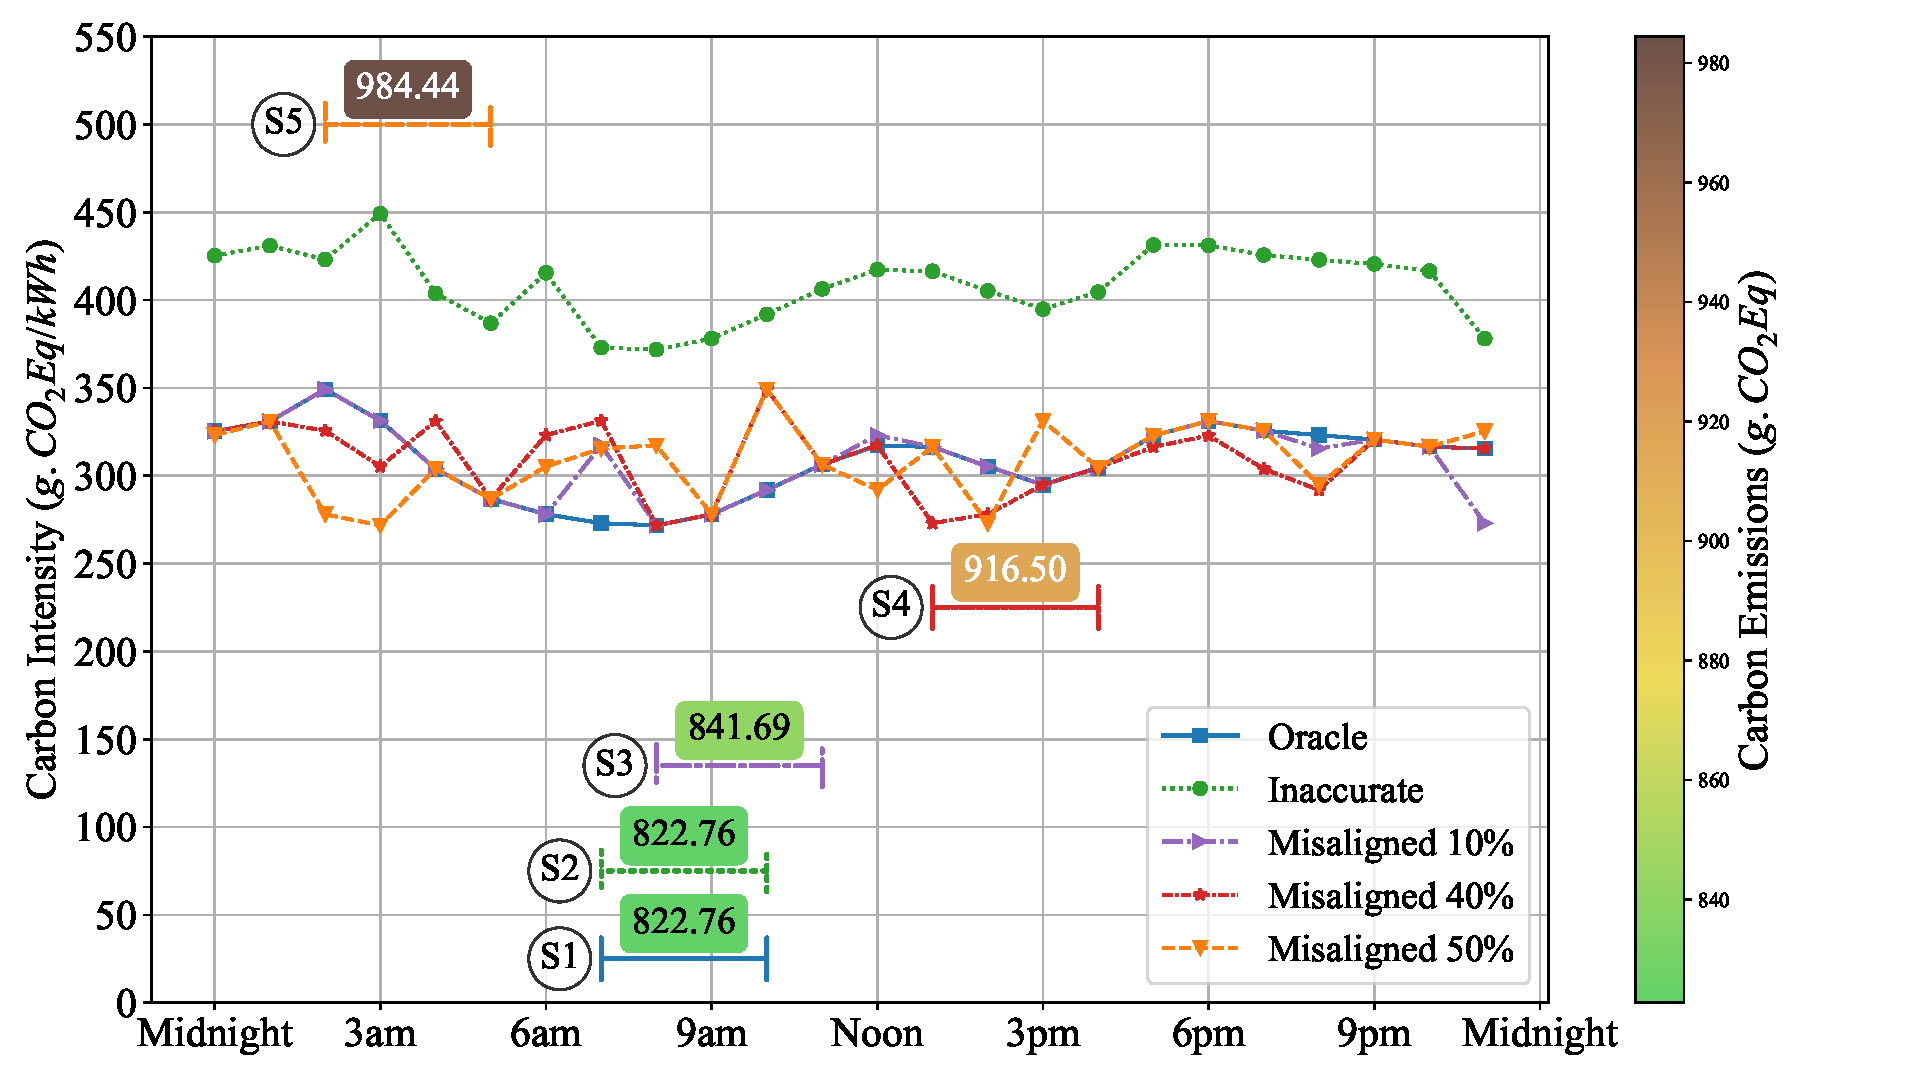
\includegraphics[width=0.85\linewidth]{images/method/MAPE_vs_Concordance_Example_in_ERCO_for_a_3_Hour_Job_Length.pdf}
    \caption{Inaccuracy versus misalignment for a 3-hour continuous job on the ERCOT grid over a 24-hour window. A high-MAPE but high-concordance forecast matches the oracle's schedule; low-MAPE forecasts with degraded concordance pick increasingly suboptimal schedules.
    \red{You need to explain this plot more in the caption. I need a sentence explaining what are the S1, S2, etc. Maybe S1 should be labeled as Sopt, while the others are numbered}}
    \label{fig:method-motivation}
\end{figure}

A forecast that is highly concordant but inaccurate can yield better scheduling outcomes than one that is accurate but poorly concordant.
Figure~\ref{fig:method-motivation} illustrates this gap between accuracy and concordance with a concrete scheduling task: a $3$-hour continuous job on the ERCOT (Texas) grid over a $24$-hour window.
Four forecasts are compared against the oracle, which identifies schedule $S_1$ at $822.76\,\text{g}\cdot\text{CO}_2\text{eq}$ as the optimum.
A deliberately ``inaccurate'' forecast with MAPE of $32\%$ nonetheless preserves the correct ordering ($C = 0.95$) and selects schedule $S_2$, achieving the same emissions as the oracle.
Three further forecasts with much lower MAPE (between $1\%$ and $5\%$) but progressively degraded concordance ($C$ falling from $0.90$ to $0.50$) select schedules $S_3$, $S_4$, and $S_5$, with realized emissions up to $20\%$ above the optimum.
The example mirrors the formal observation made in \S\ref{sec:method-formulation}: low pointwise error does not imply good scheduling, and high pointwise error does not imply bad scheduling.
What matters is whether the forecast and the ground truth agree on which hour is the cheapest.


\section{LiteCast Architecture}
\label{sec:method-litecast}

We operationalize the concordance insight with \textit{LiteCast}, a lightweight carbon-intensity forecaster and carbon-aware scheduler.
LiteCast is built on three design principles that follow directly from \S\ref{sec:method-concordance}.
First, because concordance is sensitive to the relative ordering of forecasts rather than their absolute magnitude, a model with modest accuracy but stable ordering can match or exceed accuracy-focused models in scheduling outcomes.
Second, because the relevant orderings are local in time (the window of a typical job spans hours to days), a model trained on recent data can capture them more responsively than one trained on a year of history.
% TODO: the heuristic's point is not to observe any new changes in the grid, but rather to see if we can improve the forecast during the waiting period
% Third, because grid conditions can change due to variable weather and demand, the forecaster should be cheap enough to retrain as new observations arrive between a job's submission and its scheduled start.
Third, because grid conditions can change due to variable weather and demand, the forecaster should be cheap enough to train daily to capture the changes in recent data.
% Third, because grid conditions evolve faster than long training cycles allow, the forecaster should be cheap enough to retrain as new observations arrive between a job's submission and its scheduled start.
These principles lead to a forecaster based on a classical seasonal time-series model with exogenous regressors, paired with an adaptive scheduling heuristic that exploits the model's low retraining cost.

\subsection{Architecture}
\label{sec:method-architecture}

\begin{figure}[h]
    \centering
    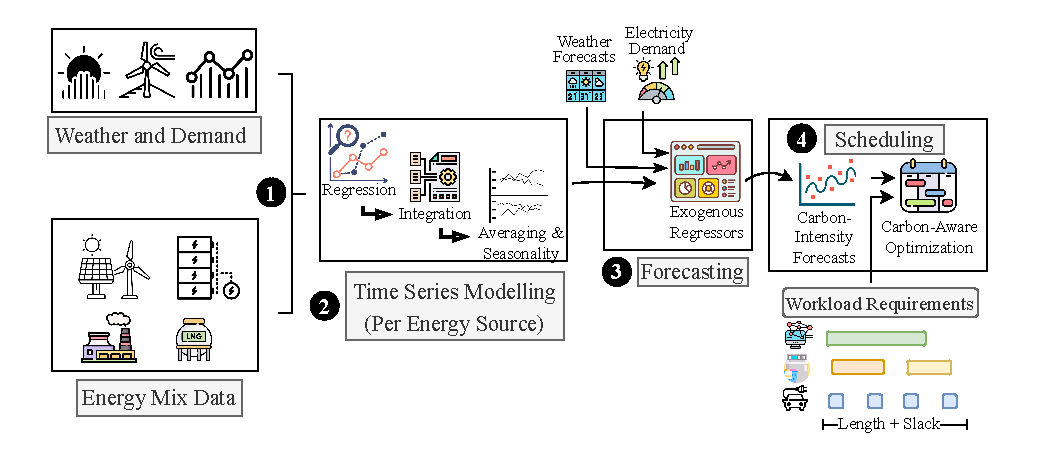
\includegraphics[width=0.95\linewidth]{images/method/litecast-v3.pdf}
    \caption{LiteCast's four-component pipeline: energy and weather data feed per-source SARIMAX models whose forecasts are aggregated into a carbon-intensity signal that drives the carbon-aware scheduler.}
    \label{fig:method-architecture}
\end{figure}

LiteCast is organized as four pipelined components, shown in Figure~\ref{fig:method-architecture}.

\begin{enumerate}
    % TODO: will need to change the seven days of data point
    \item \textbf{Energy and Weather Data.} Collects historical and forecast time series for the grid's energy mix, electricity demand, and weather variables (temperature, wind speed, solar irradiance, humidity) from public sources such as the EIA \cite{eia_data} and ENTSO-E \cite{entsoe_data}. LiteCast requires only up to a month of historical data per region, in contrast to state-of-the-art models that train on a year or more of history \cite{maji_carboncast_2022}.
    \item \textbf{Modeling.} Fits a separate time-series model for each energy source in the region's mix (e.g., coal, gas, solar, wind, nuclear), conditioned on weather and demand as exogenous regressors. The model is described in \S\ref{sec:method-model}.
    \item \textbf{Forecasting.} Generates per-source production forecasts over the requested horizon, aggregates them with the IPCC AR5 carbon factors \cite{ipcc_carbon_factors_2014} introduced in \S2.1.2, and emits an hourly average carbon-intensity forecast.
    % TODO: don't like consume
    % \item \textbf{Scheduling.} Consumes the carbon-intensity forecast together with the workload's $\mathcal{J}_{\text{length}}$ and $\mathcal{J}_{\text{slack}}$ to select a schedule via Eq.~\ref{eq:method-continuous-start} or Eq.~\ref{eq:method-interruptible-set}, and optionally invokes the adaptive heuristic of \S\ref{sec:method-heuristic}.
    \item \textbf{Scheduling.} Consumes the carbon-intensity forecast together with the workload's $\mathcal{J}_{\text{length}}$ and $\mathcal{J}_{\text{slack}}$ to select a schedule via Eq.~\ref{eq:method-continuous-start} or Eq.~\ref{eq:method-interruptible-set}.
\end{enumerate}

\subsection{Modeling}
\label{sec:method-model}

LiteCast forecasts the share of each energy source independently using SARIMAX (Seasonal AutoRegressive Integrated Moving Average with eXogenous regressors), a classical time-series model that combines four ingredients.
Autoregression captures dependence on recent past values; integration applies differencing to stabilize trends; the moving-average term captures dependence on recent forecast errors; and seasonality replicates these effects at a fixed period to model recurring daily and weekly cycles.
The exogenous regressors allow the model to condition its predictions on external drivers (i.e. weather variables, demand forecasts, hour-of-day, and day-of-week indicators) that influence each source independently of the source's own history (e.g., solar generation depends directly on solar irradiance).

% TODO: need to verify this equation 
Let $y_t$ denote the production of a single source at hour $t$, and let $\mathbf{x}_t$ denote the vector of exogenous regressors at the same hour.
LiteCast's per-source model expresses $y_t$ as
\begin{equation}
    y_t \;=\; \phi_1 \, y_{t-1} \;+\; \Phi_1 \, y_{t-24} \;-\; \Phi_1 \, y_{t-25} \;+\; \theta_1 \, \epsilon_{t-1} \;+\; \Theta_1 \, \epsilon_{t-24} \;+\; \Theta_1 \, \epsilon_{t-25} \;+\; \vec{\beta}^{\top} \mathbf{x}_t \;+\; \epsilon_t,
    \label{eq:method-sarimax}
\end{equation}
where $\phi_1$ is the non-seasonal autoregressive coefficient at lag one, $\Phi_1$ is the seasonal autoregressive coefficient at the daily lag of $24$ hours, $\theta_1$ and $\Theta_1$ are the corresponding non-seasonal and seasonal moving-average coefficients, $\vec{\beta}$ is the vector of exogenous-regressor coefficients, and $\epsilon_t$ is a zero-mean noise term.
The cross-lag terms at $t-25$ arise from differencing the seasonal component to remove the daily trend, ensuring that $y_t$ is modeled as a stationary process around its diurnal cycle.
We use the SARIMAX implementation in \texttt{statsmodels} \cite{statsmodels} and fit one model per energy source per region.

The aggregated carbon-intensity forecast is then computed by weighting each source's predicted production by its IPCC operational carbon factor and dividing by the predicted total demand:
\begin{equation}
    \hat{f}_t \;=\; \frac{\sum_{s \in \mathcal{S}} c_s \, \hat{y}_{s,t}}{\sum_{s \in \mathcal{S}} \hat{y}_{s,t}},
    \label{eq:method-aggregation}
\end{equation}
where $\mathcal{S}$ is the set of sources active in the region, $c_s$ is the operational carbon factor of source $s$ (Table~2.1), and $\hat{y}_{s,t}$ is the forecast energy production of source $s$ at hour $t$.

% It also aims to detect trends which is important for concordance
SARIMAX has three properties that align with the design principles above.
It is \textit{deterministic}: each call returns a point forecast rather than a distribution, so the relative ordering of $\hat{f}_t$ across the window is unambiguous and concordance is well-defined.
It is \textit{interpretable}: the coefficients $\phi_1$, $\Phi_1$, $\theta_1$, $\Theta_1$, and $\vec{\beta}$ have direct physical meaning, which simplifies debugging when forecasts fail in a new region. \red{How does this correlate with the design principles? Which principle? I don't see the connection. Also "simplifying debugging" is a very weak argument.}
And it is \textit{lightweight}: fitting a model on up to a month of hourly data takes seconds on a single CPU core, in contrast to the hours of GPU training required by deep-learning forecasters.
% These properties together make LiteCast cheap to retrain whenever new data arrives, which the scheduling heuristic in \S\ref{sec:method-heuristic} exploits.
These properties together make LiteCast cheap to train every day for any length of windows.

% Long-Horizon Forecasting subsection commented out: forecasting exogenous
% data over long horizons is a problem every carbon-intensity model faces,
% and LiteCast doesn't do anything novel here.
% \subsection{Long-Horizon Forecasting}
% \label{sec:method-horizon}
%
% Carbon-aware schedulers for long-running workloads -- AI training jobs, scientific simulations, geographically distributed batch pipelines -- need carbon-intensity forecasts that span days, not hours.
% The exogenous regressors in Eq.~\ref{eq:method-sarimax} (weather and demand) are themselves only available as forecasts for a limited horizon: third-party weather services typically publish forecasts up to seven days ahead, and short-term demand forecasts are commonly available for the day ahead.
% For windows that exceed the horizon at which exogenous forecasts are published, LiteCast generates the missing exogenous values by recursively forecasting them with a secondary time-series model.
% For each exogenous variable, the secondary model is selected per region as the one that achieves lower MAPE on a validation window between SARIMAX (using the same formulation as Eq.~\ref{eq:method-sarimax} but without further exogenous inputs) and Prophet, an additive decomposition model designed for long-horizon time series with multiple seasonalities.
% The chosen model produces extended forecasts of the exogenous variables, which are then fed back into Eq.~\ref{eq:method-sarimax} to extend $\hat{f}_t$ over the full window.

% \subsection{Adaptive Heuristic}
% \label{sec:method-heuristic}

% The schedule produced by Eq.~\ref{eq:method-continuous-start} or~\ref{eq:method-interruptible-set} is fixed at the moment a job arrives in the queue.
% In practice, however, the time between a job's arrival and its scheduled start can span hours or days, during which recent weather, demand, and energy-mix observations arrive that were not available at submission time.
% LiteCast exploits this gap with an adaptive heuristic that retrains the model and revises the schedule whenever the heuristic recognizes the concordance of the original forecasting is lower than expected.
% % LiteCast exploits this gap with an adaptive heuristic that retrains the model and revises the schedule whenever the new data both improves concordance and lowers projected emissions.
% The heuristic is possible entirely because of LiteCast's low retraining cost, low data requirement, and high adaptability: a deep-learning forecaster would not be able to recognize these small changes within its year long training data and dedicated infrastructure.
% % The heuristic relies entirely on LiteCast's low retraining cost: a deep-learning forecaster cannot be retrained at this cadence without dedicated infrastructure.

% Algorithm~\ref{alg:method-heuristic} formalizes the procedure.
% The heuristic operates on the window between a job's arrival and its currently scheduled start, advancing one hour at a time.
% It maintains a \textit{pseudo-oracle}: a hybrid signal that begins as a copy of the original forecast and, at each tick, has its entry for the elapsed hour overwritten with the now-known realized carbon intensity.
% The pseudo-oracle is a proxy for the true carbon intensity over the window: it agrees with $f^{\text{act}}$ on every hour that has already passed, and falls back to the original forecast for every hour still in the future.
% The future carbon intensity would be the best ground truth on when the best schedule and the quality of the forecast, but since that is not accessible at the job's arrival the heuristic uses the pseudo-oracle as its next best choice. 
% At each tick, the heuristic measures the concordance of the original forecast against this pseudo-oracle.
% While that concordance stays above $THRESHOLD$, the original forecast is still ordering the window's hours in a way that is consistent with what has actually been observed, and no action is taken.
% When the concordance drops below $THRESHOLD$, the forecast's ordering has drifted from reality, and the heuristic refits the model on a fresh training window ending at the current hour to produce a $reforecast$.
% Because committing to every reforecast would risk reacting to transient noise, the heuristic only accepts the reforecast with probability $p_1$, sampled from a Bernoulli distribution; otherwise the original schedule is kept.
% On acceptance, the schedule is recomputed over the remaining hours of the window via $\mathit{getSchedule}$ and the pseudo-oracle is reset to track the new forecast.

% \newcommand{\trainwindow}[1]{\left(#1 - train\_len,\ #1 - 1h\right)}

% \makeatletter
% \newenvironment{breakablealgorithm}
%   {\begin{center}
%      \refstepcounter{algorithm}%
%      \hrule height.8pt depth0pt \kern2pt%
%      \renewcommand{\caption}[2][\relax]{%
%        {\raggedright\textbf{\ALG@name~\thealgorithm} ##2\par}%
%        \ifx\relax##1\relax
%          \addcontentsline{loa}{algorithm}{\protect\numberline{\thealgorithm}##2}%
%        \else
%          \addcontentsline{loa}{algorithm}{\protect\numberline{\thealgorithm}##1}%
%        \fi
%        \kern2pt\hrule\kern2pt
%      }%
%   }
%   {\kern2pt\hrule\relax\end{center}}
% \makeatother

% \begin{breakablealgorithm}
% \caption{Carbon-aware scheduling heuristic with concordance-based reforecasting}
% \label{alg:method-heuristic}
% \begin{algorithmic}[1]
% \Require $j_{len},\ j_{slack},\ w_{len},\ w_{start},\ min\_train\_len$ \Comment{Job and window parameters; hourly granularity}
% \Require $THRESHOLD,\ p_0,\ p_1$ \Comment{Reforecast trigger threshold; accept/reject probabilities}
% \Require $\hat{f}((train_s, train_e),\ f_{start},\ f_{len})$ \Comment{Forecast over $[f_{start}, f_{start}+f_{len})$ trained on $[train_s, train_e]$}
% \Require $\text{oracle}(t)$,\ $\text{rand}([(a,b)])$ \Comment{True emissions; Bernoulli sampler}
% \Require $\mathit{getSchedule}(f)$,\ $\mathit{getConcordance}(a, f)$ \Comment{Best execution time; concordance under $f$}
% \Procedure{Heuristic}{}
%     \State $train\_len \gets \lceil min\_train\_len / w_{len} \rceil \times w_{len}$
%     \State $forecast \gets \hat{f}(\trainwindow{w_{start}},\ w_{start},\ w_{len})$
%     \State $scheduled\_exec \gets \mathit{getSchedule}(forecast)$
%     \State $pseudo\_oracle \gets forecast.\text{copy}()$
%     \State $cur\_time \gets w_{start}$
%     \While{$cur\_time < scheduled\_exec$}
%         \State $pseudo\_oracle[cur\_time] \gets \text{oracle}(cur\_time)$
%         \State $cur\_time \gets cur\_time + 1h$
%         \If{$\mathit{getConcordance}(forecast,\ pseudo\_oracle) < THRESHOLD$}
%             \State $reforecast \gets \hat{f}(\trainwindow{cur\_time},\ w_{start},\ w_{len})$
%             \State $reforecast[i] \gets \text{oracle}(i)\ \forall\, i \in [w_{start},\ cur\_time)$ \Comment{Replace elapsed values with oracle}
%             \If{$\text{rand}([p_0,\ p_1]) = 1$} \Comment{Accept the reforecast}
%                 \State $forecast \gets reforecast$
%                 \State $scheduled\_exec \gets \mathit{getSchedule}(forecast[cur\_time:])$
%                 \State $pseudo\_oracle \gets forecast.\text{copy}()$
%             \EndIf
%         \EndIf
%     \EndWhile
%     \State \Return $actualized\_emissions$
% \EndProcedure
% \end{algorithmic}
% \end{breakablealgorithm}

% The pseudo-oracle and the probabilistic accept step are what make the heuristic safe to apply repeatedly.
% Comparing the forecast against the pseudo-oracle, rather than against the latest individual observation, keeps the trigger anchored in the cumulative evidence of how the window has unfolded so far, so a single anomalous hour cannot by itself force a reforecast.
% The threshold $THRESHOLD$ then sets the tolerance: tighter values reforecast aggressively in the face of small ordering drifts, while looser values reserve action for clear and sustained divergence.
% The Bernoulli accept step with probability $p_1$ adds a second guard against over-reaction.
% Even when the concordance has fallen below $THRESHOLD$, the reforecast may itself be noisy or may differ from the original in ways that do not justify rescheduling.
% Accepting the reforecast only a $p_1$ fraction of the time damps oscillation between forecasts, lets $p_1$ be tuned to the volatility of the grid, and recovers the original deterministic behavior at the limits $p_1 = 0$ (never reforecast) and $p_1 = 1$ (always reforecast on threshold breach).

% \section{Summary}
% \label{sec:method-summary}

% This chapter formalized the carbon-aware scheduling problem and showed that the forecast enters realized emissions only through the schedule it selects, never through its absolute values.
% This structural property motivates concordance -- the preservation of the ordering of carbon intensities -- as the property a carbon-intensity forecaster should optimize, in place of the pointwise accuracy metrics used by prior work.
% LiteCast operationalizes the insight with a per-source SARIMAX model trained on seven days of data, an aggregated carbon-intensity forecast, and an adaptive heuristic that exploits the model's low retraining cost to revise schedules as new observations arrive.
% The next chapter evaluates LiteCast against state-of-the-art forecasters across $50$ regions and a range of workload lengths and slacks.